% !Rnw root = main.Rnw


% !Rnw root = Introduction.Rnw
%===============================
\section{The Dataset}
%===============================
\textbf{Its time to get real!!}. We give you the \textbf{``Yelp Open Dataset''} . 
For the rest of our journey, we will be presenting different data manipulation, visualization and modelling techniques using this data set as our example. The idea is to get you acquainted with  typically large, and noisy data sets as is prevalent in today's world and to show you how to explore these data sets using R. The data set has been provided to you as set of 11 files, along with this reader. The inter-relation between the attributes can be found at the end of this chapter. Further details of the data set can be found in \textcolor{cyan}{\url{https://www.yelp.com/dataset}} 

\begin{figure}[ht]
 \centering
    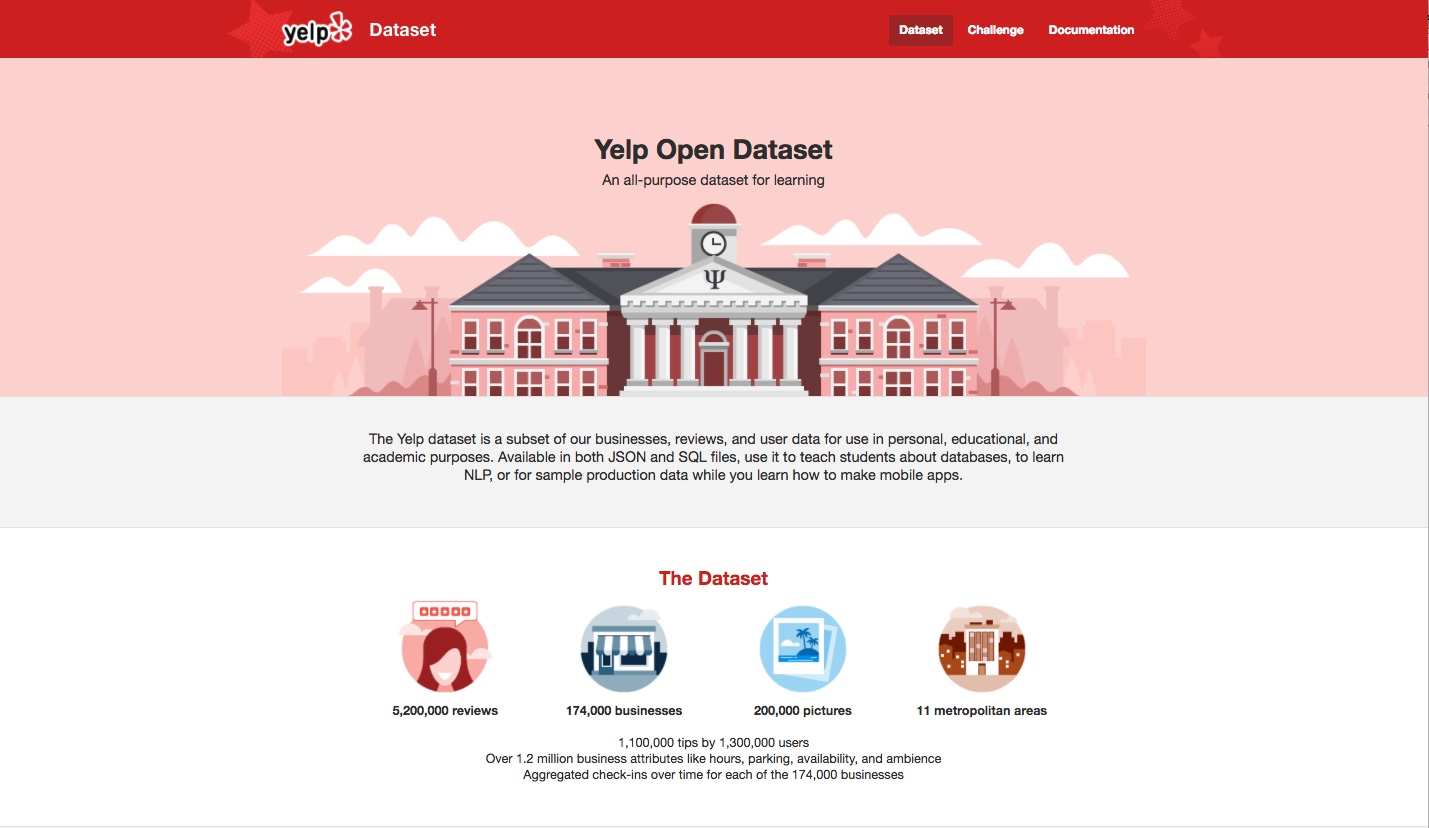
\includegraphics[ height=11cm,width = 15 cm]{./viz/ext/theYelpDataset.jpeg}
\end{figure}



% !Rnw root = Introduction.Rnw
%===============================
\section{Data Wrangling}
%===============================

\begin{HIGHLIGHT}
\par\noindent{
\noindent \textbf{\emph{Data Wrangling}} sometimes referred to as data munging, is the process of transforming and mapping data from its raw form to a form that is suitable for analysis.
Exploring data for new insights is a gradual, iterative process. Occasionally we get a sudden insight, but for the most part we try something, look at the results, reflect a bit, and then try something slightly different.
}
\end{HIGHLIGHT}

\noindent In this section, we will learn about ways to  \textbf{(a)} Clean \textbf{(b)} Transform and \textbf{(c)} Aggregate data. 
Therefore, we will formulate different questions that we wish to ask on the data and write R expressions that will enable us to answer those questions.

\subsection{The \textbf{\emph{business}} dataset}

\noindent Import the file \emph{\textbf{business.csv}} into your R environment. 


\subsubsection{Dimension and Attributes}
\noindent \textbf{\underline{Question}}: What is the size of the data?
\begin{knitrout}
\definecolor{shadecolor}{rgb}{0.969, 0.969, 0.969}\color{fgcolor}\begin{kframe}
\begin{alltt}
\hlkwd{dim}\hlstd{(business)}
\end{alltt}
\begin{verbatim}
## [1] 156639     12
\end{verbatim}
\begin{alltt}
\hlcom{##get the dimension of the data}
\end{alltt}
\end{kframe}
\end{knitrout}

\noindent \textbf{\underline{Question}}: What are the attributes?
\begin{knitrout}
\definecolor{shadecolor}{rgb}{0.969, 0.969, 0.969}\color{fgcolor}\begin{kframe}
\begin{alltt}
\hlkwd{colnames}\hlstd{(business)}
\end{alltt}
\begin{verbatim}
##  [1] "id"           "name"         "neighborhood" "address"     
##  [5] "city"         "state"        "postal_code"  "latitude"    
##  [9] "longitude"    "stars"        "review_count" "is_open"
\end{verbatim}
\begin{alltt}
\hlcom{##get the attributes of the data}
\end{alltt}
\end{kframe}
\end{knitrout}

\newpage
\subsubsection{Uni-variate Distribution}
\noindent \textbf{\underline{Question}}: What is the distribution of ratings in the data?
\begin{knitrout}
\definecolor{shadecolor}{rgb}{0.969, 0.969, 0.969}\color{fgcolor}\begin{kframe}
\begin{alltt}
\hlkwd{boxplot}\hlstd{(business}\hlopt{$}\hlstd{stars,}\hlkwc{main} \hlstd{=} \hlstr{"Distribution of Ratings"}\hlstd{)}
\end{alltt}
\end{kframe}
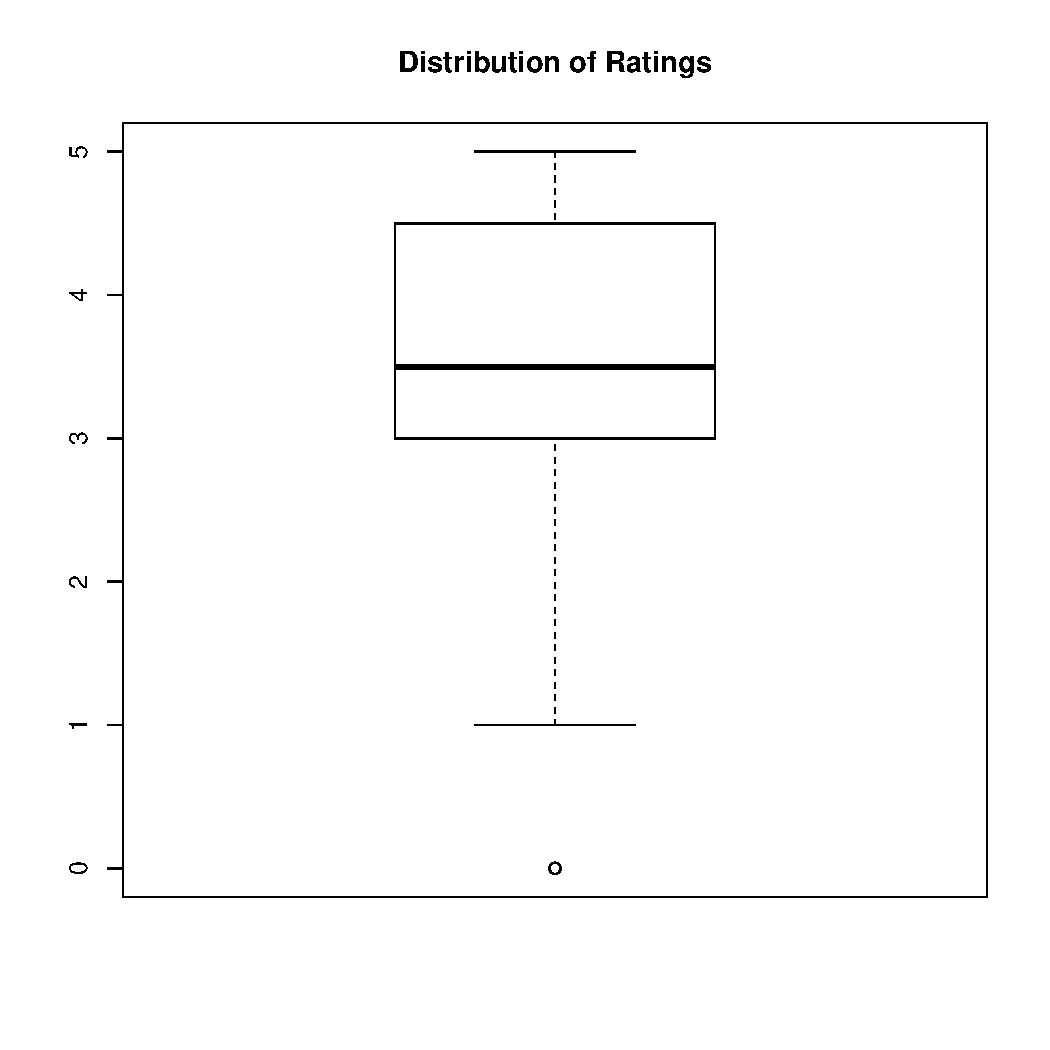
\includegraphics[width=\maxwidth]{figure/boxplotStars-1} 

\end{knitrout}

\begin{DIY}{Think}
\noindent Explain the plot
\end{DIY}

\begin{DIY}{Homework}
\noindent What is the distribution of review count in the data?
\end{DIY}

\newpage
\subsubsection{Sorting and Selection}
\noindent \textbf{\underline{Question}}: Which are the top 10 business by rating? 
\begin{knitrout}
\definecolor{shadecolor}{rgb}{0.969, 0.969, 0.969}\color{fgcolor}\begin{kframe}
\begin{alltt}
\hlkwd{head}\hlstd{(business[}\hlkwd{order}\hlstd{(business}\hlopt{$}\hlstd{stars,}
                    \hlkwc{decreasing} \hlstd{=} \hlnum{TRUE}
                    \hlstd{),}
              \hlkwd{c}\hlstd{(}\hlstr{"name"}\hlstd{,}\hlstr{"state"}\hlstd{,}\hlstr{"stars"}\hlstd{)}
              \hlstd{],}
     \hlkwc{n}\hlstd{=}\hlnum{10}\hlstd{)}
\hlcom{## sort the data by number of  stars and get the top 10 businesses}
\end{alltt}
\end{kframe}
\end{knitrout}

\begin{DIY}{Homework}
\noindent Which are the bottom 10 businesses by review count?
\end{DIY}

\subsubsection{Aggregation}
\noindent \textbf{\underline{Question}}: What is the number of business entities per state? 
\begin{knitrout}
\definecolor{shadecolor}{rgb}{0.969, 0.969, 0.969}\color{fgcolor}\begin{kframe}
\begin{alltt}
\hlstd{countPerState} \hlkwb{<-} \hlkwd{aggregate}\hlstd{(business}\hlopt{$}\hlstd{state,}
                           \hlkwc{by}\hlstd{=}\hlkwd{list}\hlstd{(business}\hlopt{$}\hlstd{state),}
                           \hlkwc{FUN}\hlstd{=length}
                           \hlstd{)}
\hlkwd{names}\hlstd{(countPerState)}\hlkwb{<-}\hlkwd{c}\hlstd{(}\hlstr{"state"}\hlstd{,}\hlstr{"count"}\hlstd{)}
\hlkwd{View}\hlstd{(countPerState)}
\hlcom{##count number of occurences of businesses in each state  }
\end{alltt}
\end{kframe}
\end{knitrout}


\begin{DIY}{Homework}
\noindent Read the help manual for the \emph{aggregate()} function.
\end{DIY}

\begin{DIY}{Think}
\noindent \begin{itemize}
  \item Why have we passed a \emph{list()} to the \textbf{by} argument? 
  \item What do you get if you just set $by = business\$state$?
\end{itemize}
\end{DIY}

\begin{DIY}{Warning}
\noindent Take a close look at the values in the \textbf{countPerState\$state} column. Do you notice any irregularities?
\end{DIY}

\newpage
\subsubsection{Filtering}
\noindent \textbf{\underline{Question}}: How can we filter out incorrect values? 
\begin{knitrout}
\definecolor{shadecolor}{rgb}{0.969, 0.969, 0.969}\color{fgcolor}\begin{kframe}
\begin{alltt}
\hlkwd{View}\hlstd{(countPerState[}\hlkwd{is.na}\hlstd{(}
                         \hlkwd{as.numeric}\hlstd{(countPerState}\hlopt{$}\hlstd{state)}
                         \hlstd{),}
                   \hlstd{]}
     \hlstd{)}
\hlcom{##filter out the entries that are of type "numeric" }
\end{alltt}
\end{kframe}
\end{knitrout}

\begin{DIY}{Think}
\noindent Explain how are we taking advantage of coercion in the above expression.
\end{DIY}

\begin{DIY}{Homework}
\noindent When we count the number of hotels per state, we see that some states are labelled as 'C'. Find the list of all businesses that belong to this state
\end{DIY}

\begin{DIY}{Homework}
\noindent The bounding box of United States in terms of (lat,lon) is (-125.0011, 24.9493) and (-66.9326, 49.5904). Find all
businesses that are located in US. Moreover, find which state in US has the highest number of 5 star businesses.
\end{DIY}

\newpage
\subsubsection{Bi-variate Distribution}
\noindent \textbf{\underline{Question}}: What is the distribution of open v/s closed business? 
\begin{knitrout}
\definecolor{shadecolor}{rgb}{0.969, 0.969, 0.969}\color{fgcolor}\begin{kframe}
\begin{alltt}
\hlkwd{table}\hlstd{(business}\hlopt{$}\hlstd{is_open)}
\hlcom{## get frequency of open v/s closed businesses }
\end{alltt}
\end{kframe}
\end{knitrout}

\begin{DIY}{Homework}
\noindent Refer to \textcolor{cyan}{\url{https://www.statmethods.net/graphs/pie.html}} and generate the pie chart as shown below
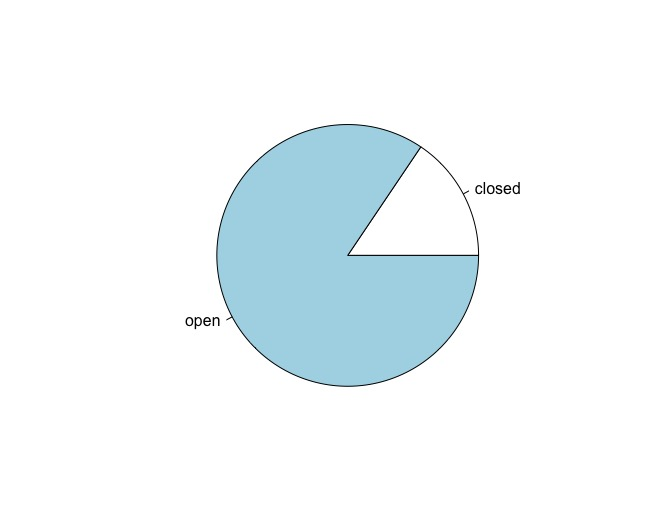
\includegraphics[width=9 cm]{./viz/ext/pieChartBusinessStatus.jpeg}
\end{DIY}


\begin{DIY}{Homework}
\noindent Refer to \textcolor{cyan}{\url{https://www.statmethods.net/graphs/boxplot.html}} and generate the boxplot as shown below. Moreover explain the plot
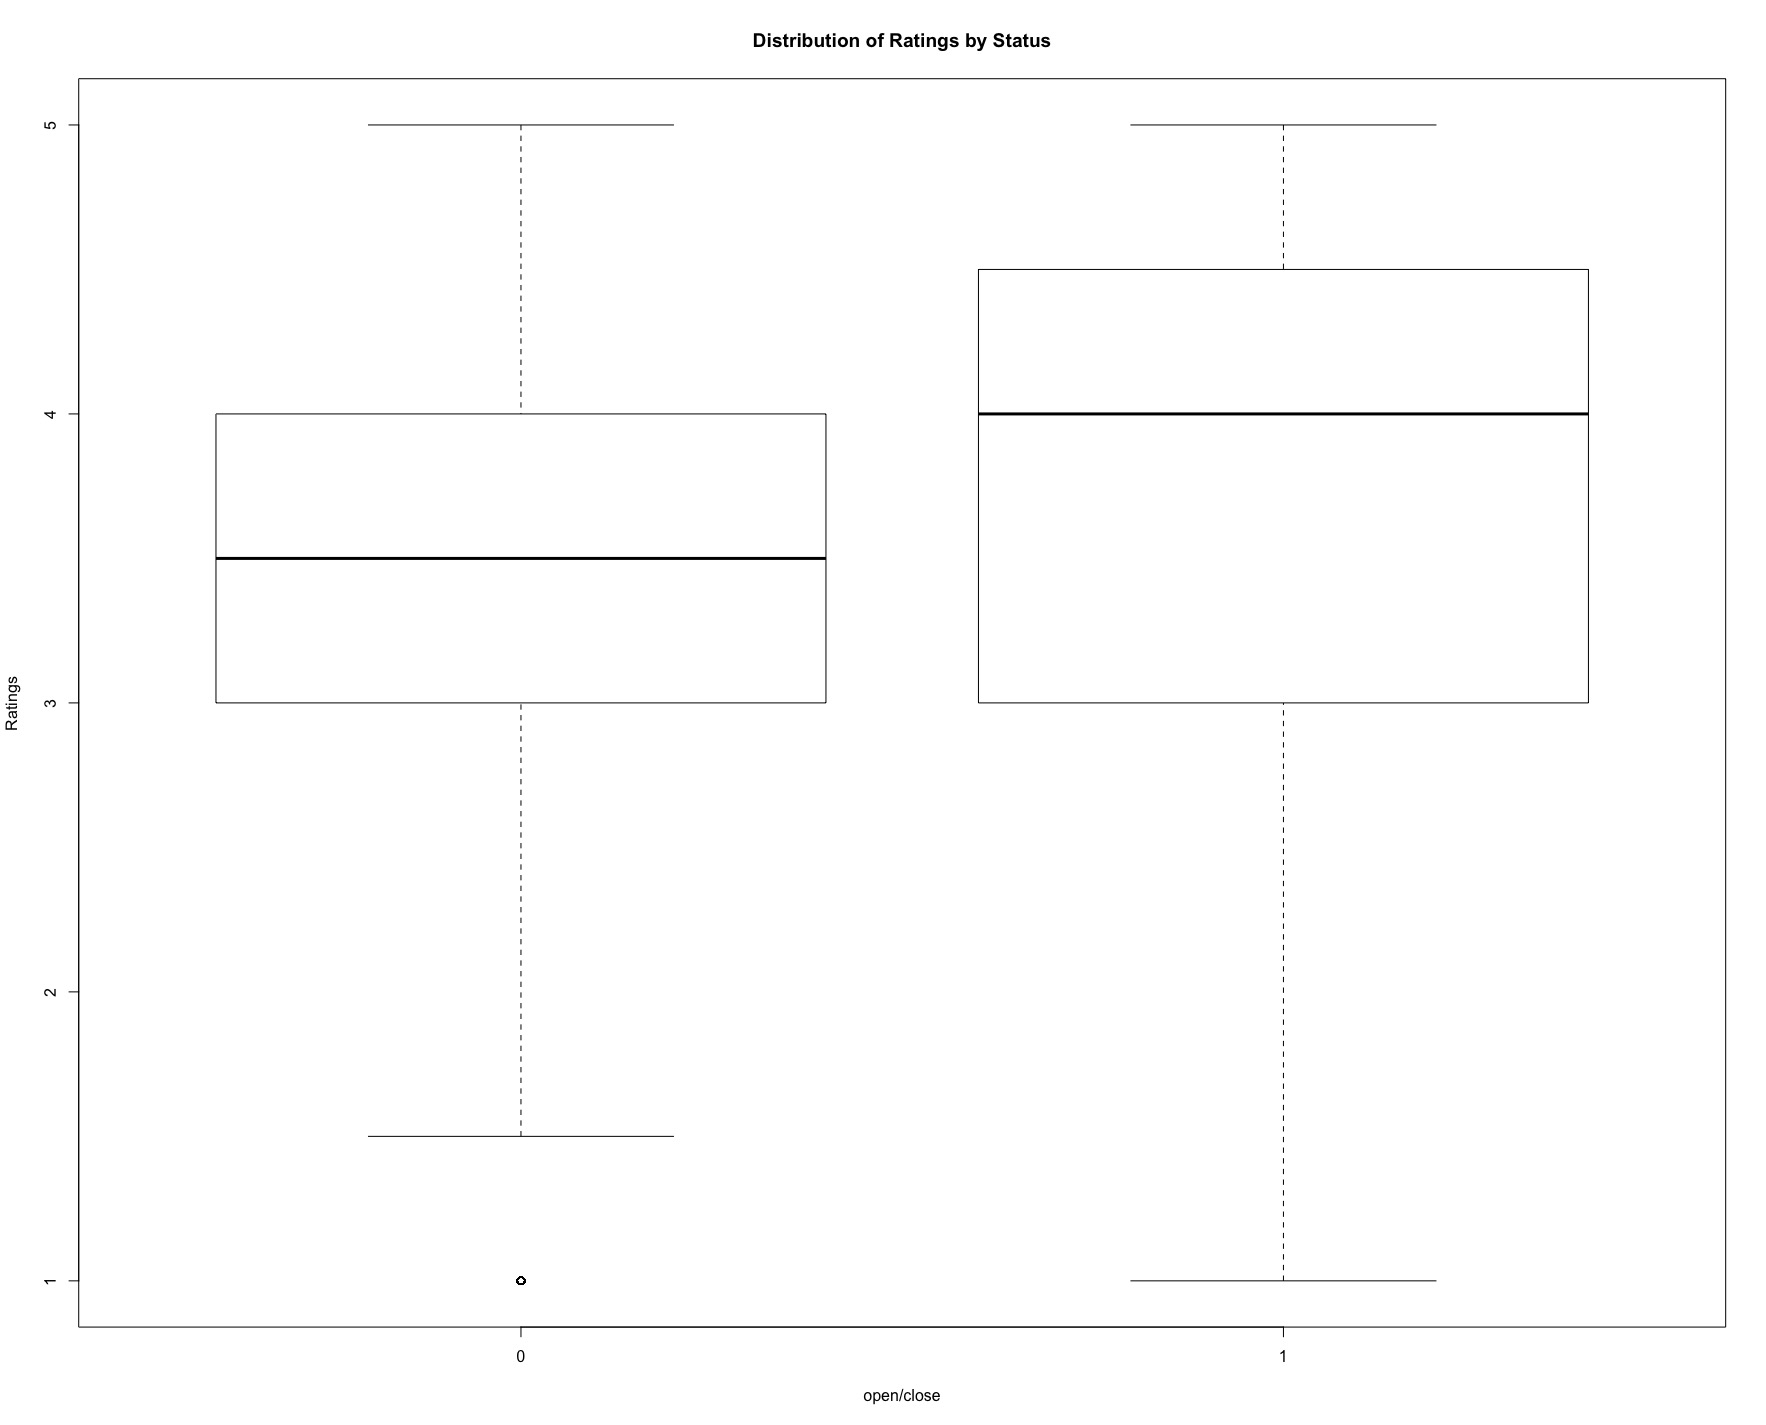
\includegraphics[width=12 cm]{./viz/ext/BoxPlot_Ratings_OpenStatus.jpeg}
\end{DIY}

\newpage
\subsubsection{Relationship among Attributes}
\noindent \textbf{\underline{Question}}: Does there exist a relationship between ratings and number of reviews?
\begin{knitrout}
\definecolor{shadecolor}{rgb}{0.969, 0.969, 0.969}\color{fgcolor}\begin{kframe}
\begin{alltt}
\hlkwd{plot}\hlstd{(business}\hlopt{$}\hlstd{review_count,business}\hlopt{$}\hlstd{stars,}
      \hlkwc{main} \hlstd{=} \hlstr{"Relation b/w review count and rating"}\hlstd{,}
     \hlkwc{xlab} \hlstd{=} \hlstr{"review_count"}\hlstd{,} \hlkwc{ylab} \hlstd{=} \hlstr{"rating"}\hlstd{)}
\end{alltt}
\end{kframe}
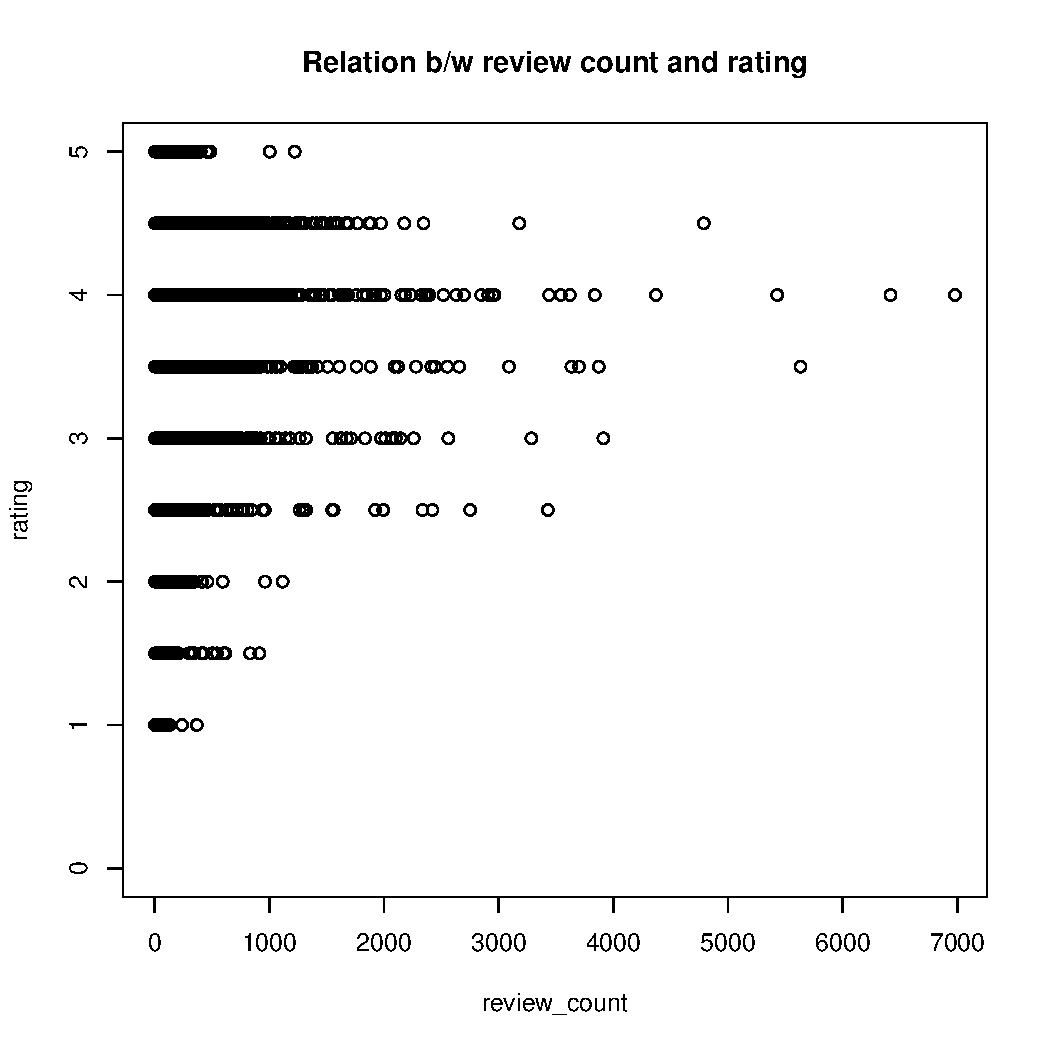
\includegraphics[width=\maxwidth]{figure/corr_Review_Stars-1} 
\begin{kframe}\begin{alltt}
\hlcom{##scatterplot of review count and ratings}
\end{alltt}
\end{kframe}
\end{knitrout}

\begin{DIY}{Think}
\noindent Explain the plot
\end{DIY}

\begin{DIY}{Homework}
\noindent Generate the scatter-plot that plots the relationship between review count and ratings for all open businesses and has number of reviews $\leq$ 1000.
\end{DIY}

\newpage
\subsection{The \textbf{\emph{category}} dataset}
\noindent Import the file \emph{\textbf{category.csv}} into your R environment.  


\subsubsection{Dimension and Attributes}
\noindent \textbf{\underline{Question}}: What is the dimension of the data and what are the various attributes?
\begin{knitrout}
\definecolor{shadecolor}{rgb}{0.969, 0.969, 0.969}\color{fgcolor}\begin{kframe}
\begin{alltt}
\hlkwd{dim}\hlstd{(category)}
\end{alltt}
\begin{verbatim}
## [1] 590290      2
\end{verbatim}
\begin{alltt}
\hlcom{##get dimension of the data}
\hlkwd{colnames}\hlstd{(category)}
\end{alltt}
\begin{verbatim}
## [1] "business_id" "category"
\end{verbatim}
\begin{alltt}
\hlcom{##get attributes of the data}
\end{alltt}
\end{kframe}
\end{knitrout}

\subsubsection{Sorting and Selection}
\noindent \textbf{\underline{Question}}: Which are the 10 most frequent categories?  
\begin{knitrout}
\definecolor{shadecolor}{rgb}{0.969, 0.969, 0.969}\color{fgcolor}\begin{kframe}
\begin{alltt}
\hlstd{countPerCategory} \hlkwb{<-} \hlkwd{aggregate}\hlstd{(category}\hlopt{$}\hlstd{category,}
                              \hlkwc{by}\hlstd{=}\hlkwd{list}\hlstd{(category}\hlopt{$}\hlstd{category),}
                              \hlstd{length}
                             \hlstd{)}
\hlcom{##count the number of occurence of each category}
\hlkwd{names}\hlstd{(countPerCategory)} \hlkwb{<-} \hlkwd{c}\hlstd{(}\hlstr{"category"}\hlstd{,}\hlstr{"count"}\hlstd{)}

\hlstd{top10Categories}\hlkwb{<-}\hlkwd{head}\hlstd{(countPerCategory[}
                            \hlkwd{order}\hlstd{(countPerCategory}\hlopt{$}\hlstd{count,}
                                  \hlkwc{decreasing} \hlstd{=} \hlnum{TRUE}
                                  \hlstd{),}
                          \hlstd{],}
         \hlkwc{n}\hlstd{=}\hlnum{10}
     \hlstd{)}
\hlcom{##sort the frequency data frame in descending order}
\hlcom{##and list the top 10}
\hlstd{top10Categories}
\end{alltt}
\end{kframe}
\end{knitrout}

\noindent \textbf{\underline{Question}}: Which business belong to the 10 most frequent categories?  
\begin{knitrout}
\definecolor{shadecolor}{rgb}{0.969, 0.969, 0.969}\color{fgcolor}\begin{kframe}
\begin{alltt}
\hlstd{businesses_top10Categories} \hlkwb{<-} \hlstd{category[category}\hlopt{$}\hlstd{category} \hlopt
                                         \hlstd{top10Categories[,}\hlnum{1}\hlstd{],]}
\hlcom{##list all entries in the category file that }
\hlcom{#belong to one of the top 10 categories}
\end{alltt}
\end{kframe}
\end{knitrout}

\begin{DIY}{Think}
\noindent How would you check if the filtering criteria applied in the last step returns the correct result
\end{DIY}

\subsubsection{Distribution of the Data}
\noindent \textbf{\underline{Question}}: Are businesses assigned to multiple categories? How many such businesses exist?
\begin{knitrout}
\definecolor{shadecolor}{rgb}{0.969, 0.969, 0.969}\color{fgcolor}\begin{kframe}
\begin{alltt}
\hlstd{businessIdFreq} \hlkwb{<-} \hlkwd{table}\hlstd{(category}\hlopt{$}\hlstd{business_id)}
\hlcom{##get number of categories each business has been assigned to}
\hlkwd{length}\hlstd{(businessIdFreq} \hlopt{>} \hlnum{0}\hlstd{)} \hlopt{>} \hlnum{0}
\end{alltt}
\begin{verbatim}
## [1] TRUE
\end{verbatim}
\begin{alltt}
\hlcom{##check if there are businesses assigned to multiple categories}
\hlkwd{plot}\hlstd{(businessIdFreq[}\hlkwd{order}\hlstd{(}
                          \hlstd{businessIdFreq,}
                          \hlkwc{decreasing} \hlstd{=} \hlnum{TRUE}
                          \hlstd{)}
                    \hlstd{],}
     \hlkwc{xlab} \hlstd{=} \hlstr{"Businesses"}\hlstd{,}
     \hlkwc{ylab}\hlstd{=}\hlstr{"Number of Assigned Categories"}\hlstd{,}
     \hlkwc{main} \hlstd{=} \hlstr{"Distribution of category assignment of businesses"}\hlstd{,}
     \hlkwc{xaxt} \hlstd{=} \hlstr{'n'}\hlstd{)}
\end{alltt}
\end{kframe}
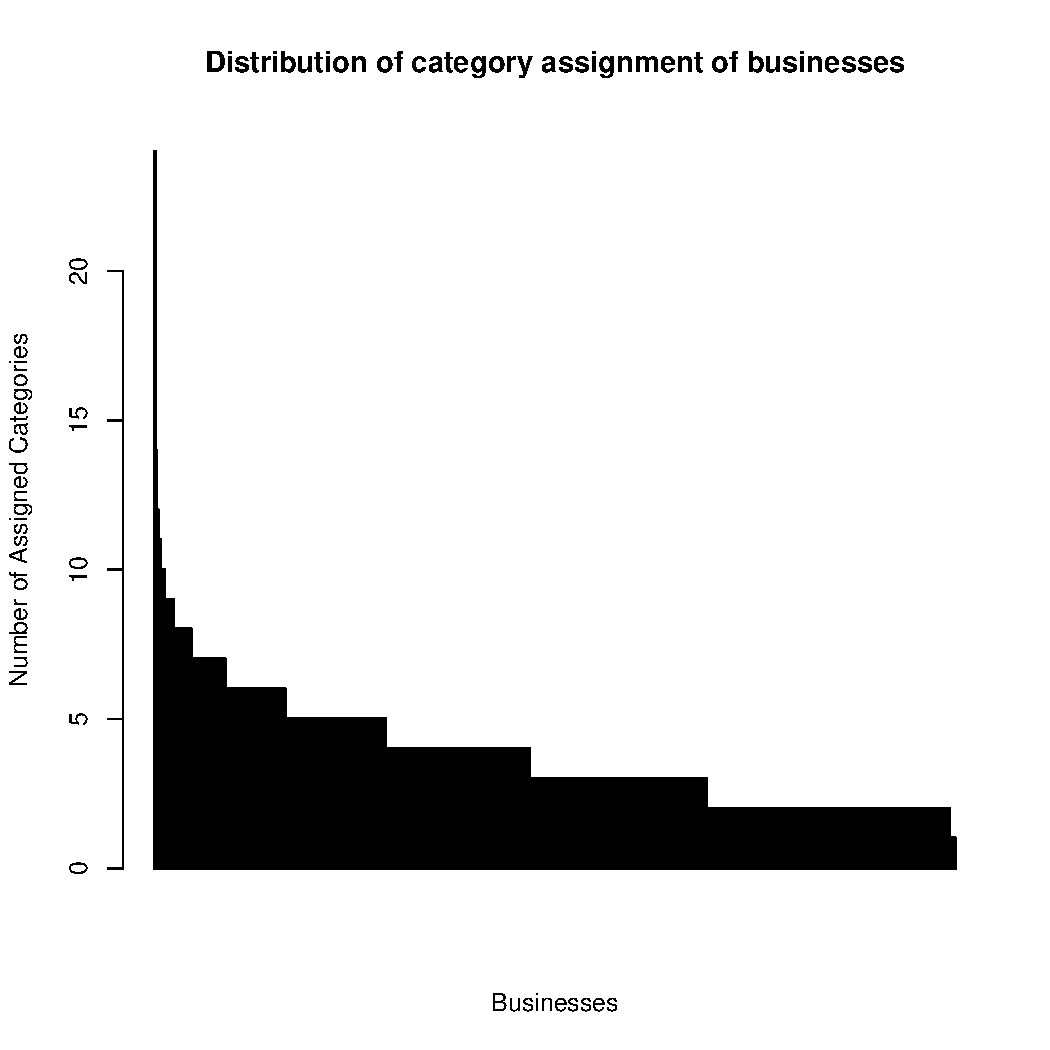
\includegraphics[width=\maxwidth]{figure/unnamed-chunk-4-1} 
\begin{kframe}\begin{alltt}
\hlcom{##sort the frequency of category assignment in descending}
\hlcom{##order and plot the same}
\end{alltt}
\end{kframe}
\end{knitrout}

\begin{DIY}{Think}
\noindent Explain the plot
\end{DIY}

\subsubsection{Joining Data sets}
\noindent \textbf{\underline{Question}}: Which business belong to the category "shopping"?  
\begin{knitrout}
\definecolor{shadecolor}{rgb}{0.969, 0.969, 0.969}\color{fgcolor}\begin{kframe}
\begin{alltt}
\hlstd{shopping} \hlkwb{<-} \hlstd{business[business}\hlopt{$}\hlstd{id} \hlopt
                        \hlstd{businesses_top10Categories}
                            \hlstd{[businesses_top10Categories}\hlopt{$}\hlstd{category}
                                \hlopt{==} \hlstr{"Shopping"}\hlstd{,}
                            \hlstd{]}\hlopt{$}\hlstd{business_id,}
         \hlstd{]}
\hlcom{##list all businesses from the business dataframe }
\hlcom{##that belong to the category "shopping"  }
\hlstd{shopping}
\end{alltt}
\end{kframe}
\end{knitrout}

\begin{DIY}{Think}
\noindent Try using 
\begin{knitrout}
\definecolor{shadecolor}{rgb}{0.969, 0.969, 0.969}\color{fgcolor}\begin{kframe}
\begin{alltt}
\hlstd{businesses_top10Categories[}
          \hlstd{businesses_top10Categories}\hlopt{$}\hlstd{category}
          \hlopt{==} \hlstr{"Shopping"}\hlstd{,}
          \hlstr{"business_id"}
          \hlstd{]}
\end{alltt}
\end{kframe}
\end{knitrout}
instead to get the list of businesses labelled with category = "Shopping". Explain the difference
\end{DIY}


\begin{DIY}{Homework}
\noindent Filter all businesses from the business data frame that belong to one of the top 10 categories
\end{DIY}

\begin{DIY}{Homework}
\noindent Calculate the average reviews count for businesses belonging to the top 10 categories and compare it against the average review count for businesses belonging to the bottom 10 categories
\end{DIY}

\subsection{The \textbf{\emph{attribute}} dataset}
\noindent Import the file \emph{\textbf{attribute.csv}} into your R environment.  


\subsubsection{Dimension and Attributes}
\noindent \textbf{\underline{Question}}: What is the dimension of the data and what are the various attributes?
\begin{knitrout}
\definecolor{shadecolor}{rgb}{0.969, 0.969, 0.969}\color{fgcolor}\begin{kframe}
\begin{alltt}
\hlkwd{dim}\hlstd{(attribute)}
\end{alltt}
\begin{verbatim}
## [1] 1229805       2
\end{verbatim}
\begin{alltt}
\hlcom{##get dimension of the data}
\hlkwd{colnames}\hlstd{(attribute)}
\end{alltt}
\begin{verbatim}
## [1] "business_id" "name"
\end{verbatim}
\begin{alltt}
\hlcom{##get attributes of the data}
\end{alltt}
\end{kframe}
\end{knitrout}

\subsubsection{Filtering, Sorting and Joining }
\noindent \textbf{\underline{Question}}: Which attributes are prevalent for restaurants with 5 star rating?
\begin{knitrout}
\definecolor{shadecolor}{rgb}{0.969, 0.969, 0.969}\color{fgcolor}\begin{kframe}
\begin{alltt}
\hlstd{fiveStarRestaurants}\hlkwb{<-}\hlstd{business[(business}\hlopt{$}\hlstd{id} \hlopt
                  \hlstd{category[}
                            \hlstd{category}\hlopt{$}\hlstd{category} \hlopt{==} \hlstr{"Restaurants"}\hlstd{,}
                         \hlstd{]}\hlopt{$}\hlstd{business_id}
          \hlstd{)}
         \hlopt{&}
         \hlstd{(business}\hlopt{$}\hlstd{stars} \hlopt{==} \hlkwd{max}\hlstd{(business}\hlopt{$}\hlstd{stars)),}
       \hlstd{]}\hlopt{$}\hlstd{id}
\hlcom{##get id's of 5 star restaurants}

\hlstd{attributeCount} \hlkwb{<-} \hlkwd{table}\hlstd{(attribute[}
                                  \hlstd{fiveStarRestaurants}
                                  \hlopt
                                  \hlstd{attribute}\hlopt{$}\hlstd{business_id,}
                                  \hlstr{"name"}\hlstd{]}
                      \hlstd{)}
\hlcom{##find attributes corresponding to the matching business }
\hlcom{##and count their number of occurences }

\hlstd{sortedAttributeCount} \hlkwb{<-} \hlstd{attributeCount[}\hlkwd{order}\hlstd{(}
                                        \hlstd{attributeCount,}
                                        \hlkwc{decreasing} \hlstd{=} \hlnum{TRUE}
                                        \hlstd{)}
                                      \hlstd{]}
\hlcom{##sort the attributes in descending order of their occurence}

\hlstd{sortedAttributePercent} \hlkwb{<-} \hlstd{sortedAttributeCount} \hlopt{/} \hlkwd{sum}\hlstd{(sortedAttributeCount)} \hlopt{*} \hlnum{100}
\hlcom{##normalize the counts                              }

\hlkwd{par}\hlstd{(}\hlkwc{las}\hlstd{=}\hlnum{2}\hlstd{)}
\hlcom{##make lable text perpendicular to the axis}

\hlkwd{par}\hlstd{(}\hlkwc{mar}\hlstd{=}\hlkwd{c}\hlstd{(}\hlnum{5}\hlstd{,}\hlnum{12}\hlstd{,}\hlnum{4}\hlstd{,}\hlnum{2}\hlstd{))}
\hlcom{##increase y-axis margin}

\hlkwd{barplot}\hlstd{(sortedAttributePercent[sortedAttributePercent} \hlopt{>} \hlnum{1}\hlstd{],}
        \hlkwc{horiz}\hlstd{=}\hlnum{TRUE}\hlstd{,}
        \hlkwc{cex.names} \hlstd{=} \hlnum{0.8}\hlstd{,}
        \hlkwc{xlab} \hlstd{=} \hlstr{"% of occurence"}\hlstd{,}
        \hlkwc{main} \hlstd{=} \hlstr{"Distribution of attributes for 5 star restaurants"}\hlstd{)}
\end{alltt}
\end{kframe}
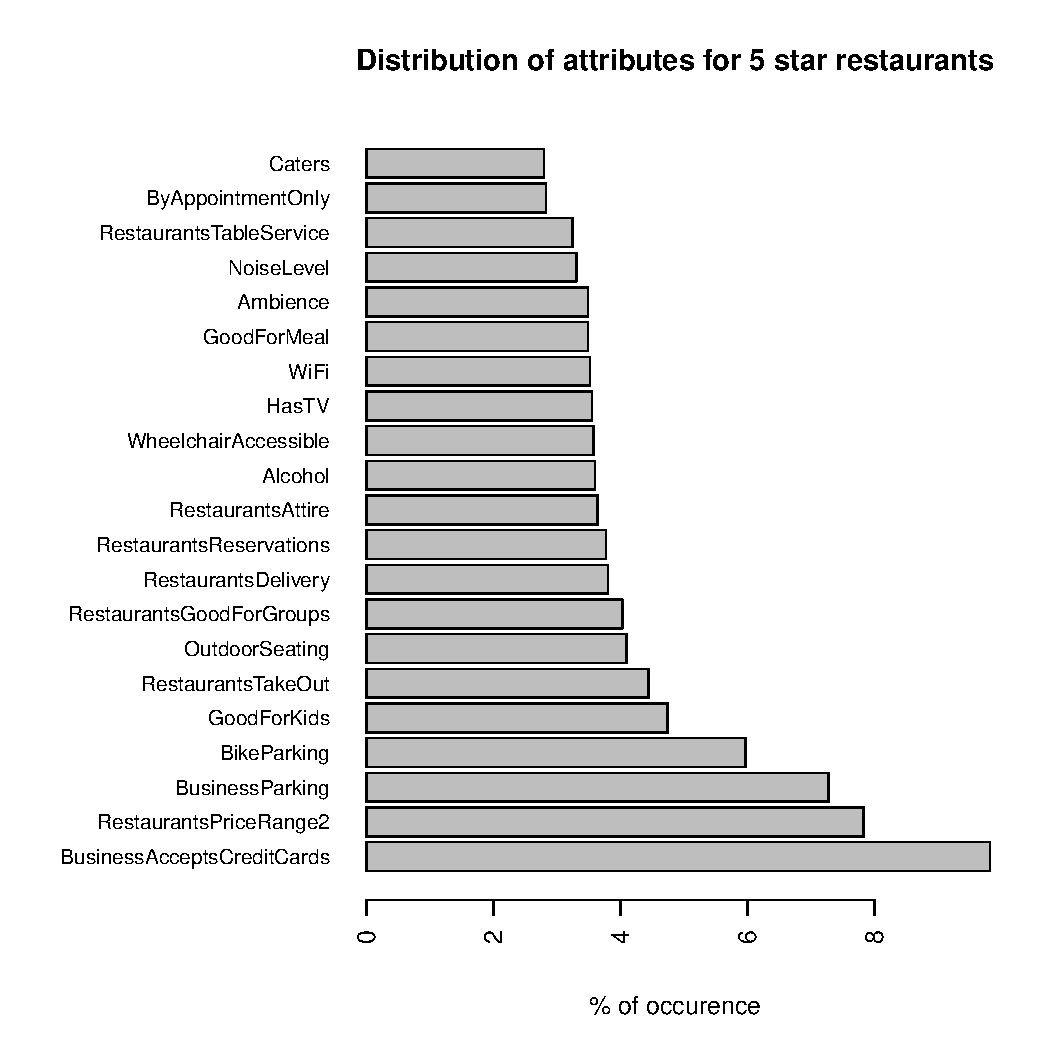
\includegraphics[width=\maxwidth]{figure/prevalentAttributes-1} 
\begin{kframe}\begin{alltt}
\hlcom{##plot the distribution of attributes }
\hlcom{##that occur at least 1% of the time}
\end{alltt}
\end{kframe}
\end{knitrout}

\begin{DIY}{Warning}
\noindent Pay close attention to the \textbf{\emph{par()}} function in the example
\end{DIY}

\begin{DIY}{Homework}
\noindent Read the help manual of the \textbf{\emph{par()}} function
\end{DIY}

\begin{DIY}{Homework}
\noindent\begin{itemize}
  \item Which attributes are prevalent for restaurants with 3 star rating? Compare the same with attributes of restaurants that have a rating of 5 stars. Explain your observation
  \item Do the same analysis for businesses which have category as "Shopping" 
\end{itemize}
\end{DIY}


%\subsection{dplyr}
%\subsection{data.table}

%<<DataVisualization,child='./DataVisualization.Rnw'>>=
%@


% !Rnw root = Introduction.Rnw
\newpage
%===============================
\section{Control Structures}
%===============================

\subsection{The \textbf{\emph{checkin}} dataset}
\noindent Import the file \emph{\textbf{checkin.csv}} into your R environment. 


\subsubsection{Dimension and Attributes}
\noindent \textbf{\underline{Question}}: What is the dimension of the data and what are the various attributes?
\begin{knitrout}
\definecolor{shadecolor}{rgb}{0.969, 0.969, 0.969}\color{fgcolor}\begin{kframe}
\begin{alltt}
\hlkwd{dim}\hlstd{(checkin)}
\end{alltt}
\begin{verbatim}
## [1] 3738750       3
\end{verbatim}
\begin{alltt}
\hlcom{##get dimension of the data}
\hlkwd{colnames}\hlstd{(checkin)}
\end{alltt}
\begin{verbatim}
## [1] "business_id" "date"        "count"
\end{verbatim}
\begin{alltt}
\hlcom{##get attributes of the data}
\end{alltt}
\end{kframe}
\end{knitrout}

\subsubsection{Splitting Strings}
\noindent \textbf{\underline{Question}}: How can we split the checkin date (DayOfWeek-HH:MM) into "day of week" and "time"?
\begin{knitrout}
\definecolor{shadecolor}{rgb}{0.969, 0.969, 0.969}\color{fgcolor}\begin{kframe}
\begin{alltt}
\hlstd{checkinTime} \hlkwb{<-} \hlkwd{strsplit}\hlstd{(checkin}\hlopt{$}\hlstd{date,}\hlkwc{split} \hlstd{=} \hlstr{"-"}\hlstd{)}
\hlcom{## split the date string into day of week and time}
\end{alltt}
\end{kframe}
\end{knitrout}

\begin{DIY}{Homework}
\noindent Read the help manual of the \textbf{\emph{strsplit()}} function
\end{DIY}

\begin{DIY}{Think}
\noindent What is the type of the object "checkinTime"? 
\end{DIY}

\newpage
\subsection{The \textbf{\emph{for}} loop}
\begin{HIGHLIGHT}
\par\noindent{
{\centering\textbf{\emph{for(name in range) body}} \\}
}
\end{HIGHLIGHT}

\subsubsection{Iterative Vectorization}
\noindent \textbf{\underline{Question}}: How can we create three vectors for "day of week", "hour of day" and "minutes" respectively?
\begin{knitrout}
\definecolor{shadecolor}{rgb}{0.969, 0.969, 0.969}\color{fgcolor}\begin{kframe}
\begin{alltt}
\hlstd{numCheckins} \hlkwb{<-} \hlkwd{length}\hlstd{(checkinTime)}
\hlcom{##the length of the list that contains }
\hlcom{## lists of the form [[<day of week>,<hour of day>,<minute>],..] }
\hlstd{dow} \hlkwb{<-} \hlkwd{vector}\hlstd{(}\hlkwc{mode} \hlstd{=} \hlstr{"character"}\hlstd{,} \hlkwc{length} \hlstd{= numCheckins)}
\hlcom{## a character vector of size = numCheckins}
\hlstd{hod} \hlkwb{<-} \hlkwd{vector}\hlstd{(}\hlkwc{mode} \hlstd{=} \hlstr{"integer"}\hlstd{,} \hlkwc{length} \hlstd{= numCheckins)}
\hlcom{## an integer vector of size = numCheckins}
\hlstd{minute} \hlkwb{<-} \hlkwd{vector}\hlstd{(}\hlkwc{mode} \hlstd{=} \hlstr{"integer"}\hlstd{,} \hlkwc{length} \hlstd{= numCheckins)}
\hlcom{## an integer vector of size = numCheckins}
\hlstd{index} \hlkwb{=} \hlnum{1} \hlcom{##set increment counter to 1}
\hlkwa{for} \hlstd{(dayTime} \hlkwa{in} \hlstd{checkinTime)\{}
      \hlcom{## iterateve over each list in the list}
      \hlstd{dow[index]}\hlkwb{<-}\hlstd{dayTime[}\hlnum{1}\hlstd{]}
      \hlcom{## extract the first element of the list (day of week)}
      \hlcom{## and assign it to the corresponding position in dow}
      \hlstd{HH_MM_split} \hlkwb{<-} \hlkwd{strsplit}\hlstd{(dayTime[}\hlnum{2}\hlstd{],}\hlkwc{split} \hlstd{=} \hlstr{":"}\hlstd{)}
      \hlcom{## split the second element }
      \hlcom{## of the list (HH:MM) into HH and MM which in turn }
      \hlcom{##creates a list of lists}
      \hlstd{hod[index]} \hlkwb{<-} \hlkwd{as.integer}\hlstd{(HH_MM_split[[}\hlnum{1}\hlstd{]][}\hlnum{1}\hlstd{])}
      \hlcom{##access the first element (hour)}
      \hlcom{## of the list of lists  and assign it to the }
      \hlcom{##corresponding position in hod}
      \hlstd{minute[index]} \hlkwb{<-} \hlkwd{as.integer}\hlstd{(HH_MM_split[[}\hlnum{1}\hlstd{]][}\hlnum{2}\hlstd{])}
      \hlcom{##access the second element (minute)}
      \hlcom{## of the list of lists and assign it to the }
      \hlcom{##corresponding position in minute}
      \hlstd{index} \hlkwb{=} \hlstd{index} \hlopt{+} \hlnum{1} \hlcom{##increment the value of index}
\hlstd{\}}
\hlstd{index} \hlkwb{=} \hlnum{1} \hlcom{##reset index to 1}
\end{alltt}
\end{kframe}
\end{knitrout}

\begin{DIY}{Think}
\begin{itemize}
  \item \noindent Explain the meaning of the \textbf{[[]]} in the context of the example
  \item \noindent What happens if we set the mode of the vectors "hod" and "minute" to \textbf{\emph{numeric}}?
\end{itemize}
\end{DIY}

\begin{DIY}{Homework}
 \begin{itemize}
  \item \noindent Install the package \textbf{rbenchmark} and read the help manual for the \textbf{\emph{benchmark()}} function.
  \item \noindent Try the above example without initializing the length/type of the vector. Benchmark the same against the given example. Explain why do you see a difference in the execution time
  \item \noindent Do not reset the index value to 1 at the end of the example and run the code block twice. Observe the size of the vectors "dow", "hod" and "minute". Explain your observation.  
\end{itemize}
\end{DIY}

\subsection{The \textbf{\emph{if}} statement}
\begin{HIGHLIGHT}
\par\noindent{
{\centering\textbf{\emph{if(test) expression1 else expression2}} \\}
}
\end{HIGHLIGHT}

\subsubsection{Conditional Assignment}
\noindent \textbf{\underline{Question}}: How can we map days of week to their position in the week? e.g. Sunday = 0, Monday = 1, $....$
\begin{knitrout}
\definecolor{shadecolor}{rgb}{0.969, 0.969, 0.969}\color{fgcolor}\begin{kframe}
\begin{alltt}
\hlstd{pow} \hlkwb{<-} \hlkwd{vector}\hlstd{(}\hlkwc{mode} \hlstd{=} \hlstr{"integer"}\hlstd{,} \hlkwc{length} \hlstd{=} \hlkwd{length}\hlstd{(dow))}
\hlcom{## create a vector of type integer where the length is }
\hlcom{## equal to the number of elements in the dow}
\hlstd{index} \hlkwb{=} \hlnum{1} \hlcom{## set the increment counter to 1}
\hlkwa{for}\hlstd{(item} \hlkwa{in} \hlstd{dow)\{} \hlcom{##iterate over element of the the }
  \hlcom{## day of week vector}
       \hlkwa{if} \hlstd{(item} \hlopt{==} \hlstr{"Sunday"}\hlstd{)\{}
         \hlstd{pow[index]} \hlkwb{<-} \hlnum{0} \hlcom{## if the day of week is sunday assign}
         \hlcom{## value 0 to the corresponding position in the pow vector}
      \hlstd{\}}
      \hlkwa{if} \hlstd{(item} \hlopt{==} \hlstr{"Monday"}\hlstd{)\{}
         \hlstd{pow[index]} \hlkwb{<-} \hlnum{1} \hlcom{## if the day of week is monday assign}
         \hlcom{## value 1 to the corresponding position in the pow vector}
      \hlstd{\}}
      \hlkwa{else if} \hlstd{(item} \hlopt{==} \hlstr{"Tuesday"}\hlstd{)\{}
         \hlstd{pow[index]} \hlkwb{<-} \hlnum{2} \hlcom{## if the day of week is tuesday assign}
         \hlcom{## value 2 to the corresponding position in the pow vector}
      \hlstd{\}}
      \hlkwa{else if} \hlstd{(item} \hlopt{==} \hlstr{"Wednesday"}\hlstd{)\{}
         \hlstd{pow[index]} \hlkwb{<-} \hlnum{3} \hlcom{## if the day of week is wednesday assign}
         \hlcom{## value 3 to the corresponding position in the pow vector}
      \hlstd{\}}
      \hlkwa{else if} \hlstd{(item} \hlopt{==} \hlstr{"Thursday"}\hlstd{)\{}
         \hlstd{pow[index]} \hlkwb{<-} \hlnum{4} \hlcom{## if the day of week is thursday assign}
         \hlcom{## value 4 to the corresponding position in the pow vector}
      \hlstd{\}}
     \hlkwa{else if} \hlstd{(item} \hlopt{==} \hlstr{"Friday"}\hlstd{)\{}
         \hlstd{pow[index]} \hlkwb{<-} \hlnum{5} \hlcom{## if the day of week is friday assign}
         \hlcom{## value 5 to the corresponding position in the pow vector}
     \hlstd{\}}
     \hlkwa{else if} \hlstd{(item} \hlopt{==} \hlstr{"Saturday"}\hlstd{)\{}
         \hlstd{pow[index]} \hlkwb{<-} \hlnum{6} \hlcom{## if the day of week is saturday assign}
         \hlcom{## value 6 to the corresponding position in the pow vector}
     \hlstd{\}}
     \hlstd{index} \hlkwb{=} \hlstd{index} \hlopt{+} \hlnum{1} \hlcom{##increment the value of index}
\hlstd{\}}
\hlstd{index} \hlkwb{=} \hlnum{1}  \hlcom{##reset index to 1}
\end{alltt}
\end{kframe}
\end{knitrout}





\begin{DIY}{Homework}
 \begin{itemize}
  \item \noindent How can you achieve the same result without using the \emph{for loop} and \emph{if statement} at all! \textcolor{red}{Hint:} try the \textbf{\emph{which()}} function. Benchmark your implementation (without the control statements) against the example. Do you notice a difference in performance? Explain your observation.
  \item \noindent Create a data frame named \emph{checkins} that has the following attributes
\end{itemize}
\end{DIY}

\begin{knitrout}
\definecolor{shadecolor}{rgb}{0.969, 0.969, 0.969}\color{fgcolor}\begin{kframe}
\begin{alltt}
 \hlkwd{colnames}\hlstd{(checkins)}
\end{alltt}
\begin{verbatim}
## [1] "business_id"      "day_of_week"      "position_of_week"
## [4] "hour"             "minute"           "count"
\end{verbatim}
\end{kframe}
\end{knitrout}

\subsubsection{Validation}
\noindent \textbf{\underline{Question}}: How can we check for correct assignment of position to day of week?
\begin{knitrout}
\definecolor{shadecolor}{rgb}{0.969, 0.969, 0.969}\color{fgcolor}\begin{kframe}
\begin{alltt}
\hlkwd{table}\hlstd{(checkins}\hlopt{$}\hlstd{day_of_week,checkins}\hlopt{$}\hlstd{position_of_week)}
\end{alltt}
\begin{verbatim}
##            
##                  0      1      2      3      4      5      6
##   Friday         0      0      0      0      0 558419      0
##   Monday         0 478652      0      0      0      0      0
##   Saturday       0      0      0      0      0      0 624409
##   Sunday    542932      0      0      0      0      0      0
##   Thursday       0      0      0      0 520651      0      0
##   Tuesday        0      0 499441      0      0      0      0
##   Wednesday      0      0      0 514246      0      0      0
\end{verbatim}
\begin{alltt}
\hlcom{##co-occurence count of day of week and position}
\hlkwd{sum}\hlstd{(}\hlkwd{table}\hlstd{(checkins}\hlopt{$}\hlstd{day_of_week,checkins}\hlopt{$}\hlstd{position_of_week))} \hlopt{==}
  \hlkwd{dim}\hlstd{(checkins)[}\hlnum{1}\hlstd{]}
\end{alltt}
\begin{verbatim}
## [1] TRUE
\end{verbatim}
\begin{alltt}
\hlcom{##check if every day of week has been mapped to one position}
\end{alltt}
\end{kframe}
\end{knitrout}

\begin{DIY}{Think}
\noindent Explain the output of the code snippet 
\end{DIY}

\begin{DIY}{Homework}
\noindent Compute the total number of checkins aggregated by hour and day of week. Plot the same 
\end{DIY}

\newpage
\subsubsection{Conditional Distribution}
\noindent \textbf{\underline{Question}}: What is the distribution of checkins over each day of the week?
\begin{knitrout}
\definecolor{shadecolor}{rgb}{0.969, 0.969, 0.969}\color{fgcolor}\begin{kframe}
\begin{alltt}
\hlkwd{summary}\hlstd{(checkins}\hlopt{$}\hlstd{count)}
\end{alltt}
\begin{verbatim}
##    Min. 1st Qu.  Median    Mean 3rd Qu.    Max. 
##    1.00    1.00    2.00    4.23    3.00 1420.00
\end{verbatim}
\begin{alltt}
\hlcom{##generate summary statistic for checkin count}
\hlkwd{boxplot}\hlstd{(checkins}\hlopt{$}\hlstd{count} \hlopt{~} \hlstd{checkins}\hlopt{$}\hlstd{day_of_week,}
        \hlkwc{main} \hlstd{=} \hlstr{"Distribution of checkins over days of week"}\hlstd{,}
        \hlkwc{xlab} \hlstd{=} \hlstr{"day of week"}\hlstd{,}\hlkwc{ylab} \hlstd{=} \hlstr{"Number of checkins"}\hlstd{)}
\end{alltt}
\end{kframe}
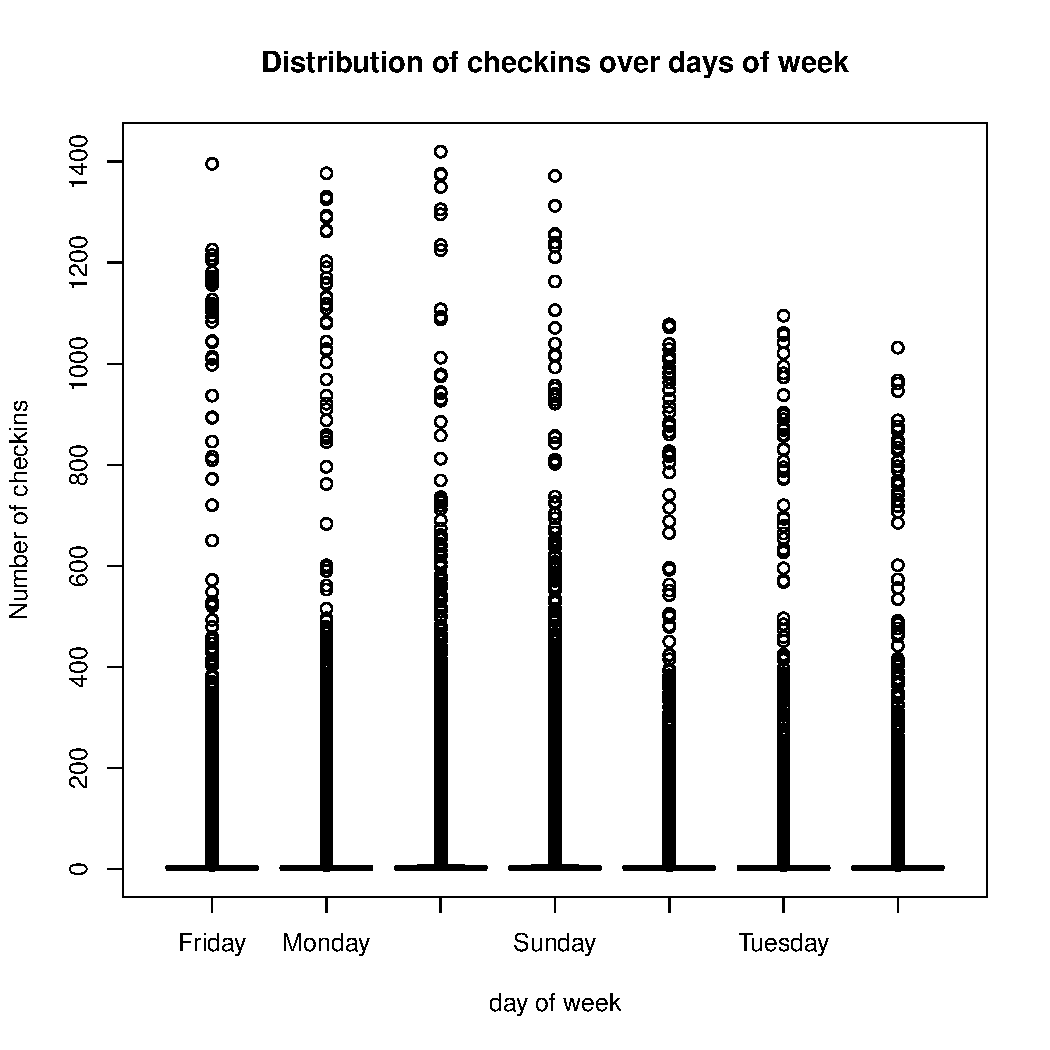
\includegraphics[width=\maxwidth]{figure/checkinsOverWeek-1} 
\begin{kframe}\begin{alltt}
\hlcom{##distribution of count , given, day of week}
\end{alltt}
\end{kframe}
\end{knitrout}

\begin{DIY}{Think}
\noindent Explain the plot
\end{DIY}

\begin{DIY}{Homework}
\begin{itemize}
  \item \noindent Regenerate the plot but only for checkins $\geq$ 3rd Quartile
  \item \noindent Generate a plot that shows the relationship between hour of day and number of checkins. Explain if you notice a relationship between the two
\end{itemize}
\end{DIY}


% !Rnw root = Introduction.Rnw
\newpage
%===============================
\section{Functions}
%===============================
\begin{HIGHLIGHT}
\par\noindent{
{\centering\textbf{function(arguments) body} \\}
}
\end{HIGHLIGHT}
\noindent \textbf{\underline{Question}}: How can we split the "date" attribute into "day of week", "hour of day" and "minutes" respectively?
\begin{knitrout}
\definecolor{shadecolor}{rgb}{0.969, 0.969, 0.969}\color{fgcolor}\begin{kframe}
\begin{alltt}
\hlcom{## a generic splitting function that accepts as arguments}
\hlcom{## - an input of type characer that is to be split }
\hlcom{## - the delimiter for day}
\hlcom{## - the delimiter for time}
\hlcom{## returns : a list of the form }
\hlcom{##           [<day of week>, <hour of day>, <minute>]}
\hlstd{getDOW_HOD} \hlkwb{<-} \hlkwa{function}\hlstd{(}\hlkwc{dateString}\hlstd{,}\hlkwc{dowSplitter} \hlstd{=} \hlstr{""}\hlstd{,}\hlkwc{timeSplitter} \hlstd{=} \hlstr{""}\hlstd{)\{}
            \hlstd{splitValues} \hlkwb{<-} \hlkwd{strsplit}\hlstd{(dateString,}\hlkwc{split} \hlstd{= dowSplitter)}
            \hlstd{dow} \hlkwb{<-} \hlstd{splitValues[[}\hlnum{1}\hlstd{]][}\hlnum{1}\hlstd{]}
            \hlstd{HH_MM_split} \hlkwb{<-} \hlkwd{strsplit}\hlstd{(splitValues[[}\hlnum{1}\hlstd{]][}\hlnum{2}\hlstd{],}
                                    \hlkwc{split} \hlstd{= timeSplitter)}
            \hlstd{hod} \hlkwb{<-} \hlkwd{as.numeric}\hlstd{(HH_MM_split[[}\hlnum{1}\hlstd{]][}\hlnum{1}\hlstd{])}
            \hlstd{mod} \hlkwb{<-} \hlkwd{as.numeric}\hlstd{(HH_MM_split[[}\hlnum{1}\hlstd{]][}\hlnum{2}\hlstd{])}
            \hlkwd{return}\hlstd{(}\hlkwd{list}\hlstd{(}\hlkwc{dayOfWeek} \hlstd{= dow,}
                        \hlkwc{hourOfDay} \hlstd{= hod,}
                        \hlkwc{minute} \hlstd{= mod))}
\hlstd{\}}

\hlcom{## for every elment in checkin\textbackslash{}$date apply the }
\hlcom{## function getDOW_HOD}
\hlstd{result} \hlkwb{<-} \hlkwd{lapply}\hlstd{(checkin}\hlopt{$}\hlstd{date,}
                 \hlstd{getDOW_HOD,}
                 \hlkwc{dowSplitter} \hlstd{=} \hlstr{'-'}\hlstd{,}\hlkwc{timeSplitter} \hlstd{=} \hlstr{':'}
                \hlstd{)}
\end{alltt}
\end{kframe}
\end{knitrout}

\begin{DIY}{Think}
\noindent Read the help manual for \textbf{\emph{lapply()}}. Try using \textbf{\emph{apply()}} instead of \textbf{\emph{lapply()}}.
\end{DIY}

\begin{DIY}{Warning}
\textcolor{red}{The reader is urged to work on the following exercise!}
\end{DIY}

\begin{DIY}{Homework}
\noindent \textcolor{red}{Write a R function that:} Given a category and time of week e.g (weekday/weekend),(morning/evening), the function should compute the number of checkins per state. Moreover, the function should also check if there exists a relationship between the rating of a business and the number of checkins 
The function should also generate plots that visualize the results.
\end{DIY}


